A reliable control policy lies at the heart of any robotic locomotion system, acting as the decision-making mechanism that translates high-level objectives into low-level motor commands. The first step is selecting a suitable environment, where the primary focus is on replicating physical constraints while allowing for iterative training. In many cases, this environment can be a simulator equipped with detailed robot models, such as those derived from URDF files, which define the geometry and dynamics of the robotic system. By running experiments in a controlled and often accelerated environment, researchers can quickly gather feedback on different policy configurations while reducing the risk of hardware damage. The simulator can also be augmented with sensor data and randomization factors to expose the policy to varied conditions, promoting robustness that will extend beyond the simulator.

\begin{figure}[htbp]
	\centering
	\begin{subfigure}{0.45\linewidth}
		\centering
		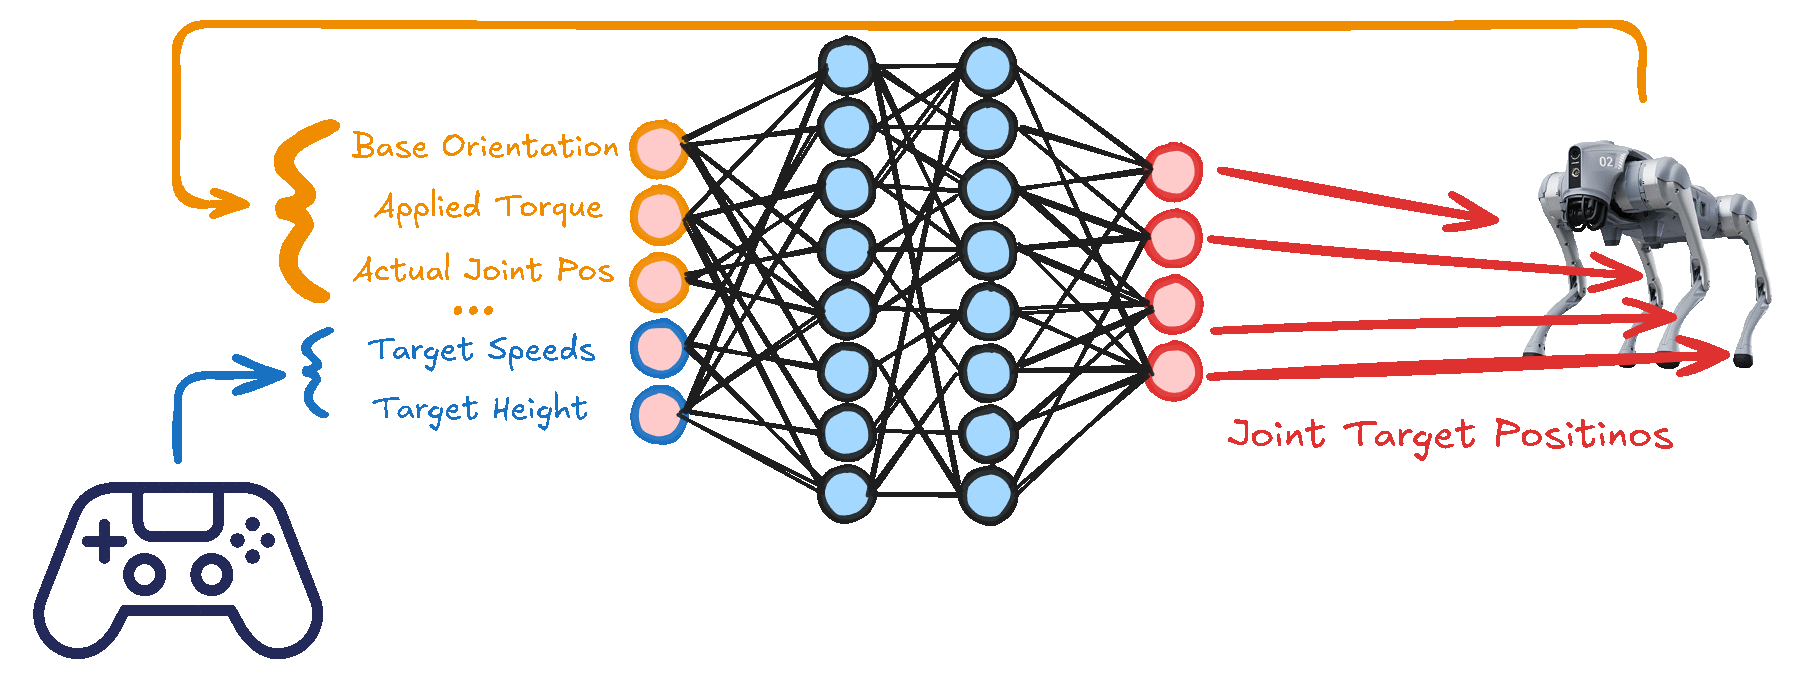
\includegraphics[width=0.9\linewidth]{fig/policyaa_1}
	\end{subfigure}
	\centering
	\begin{subfigure}{0.45\linewidth}
		\centering
		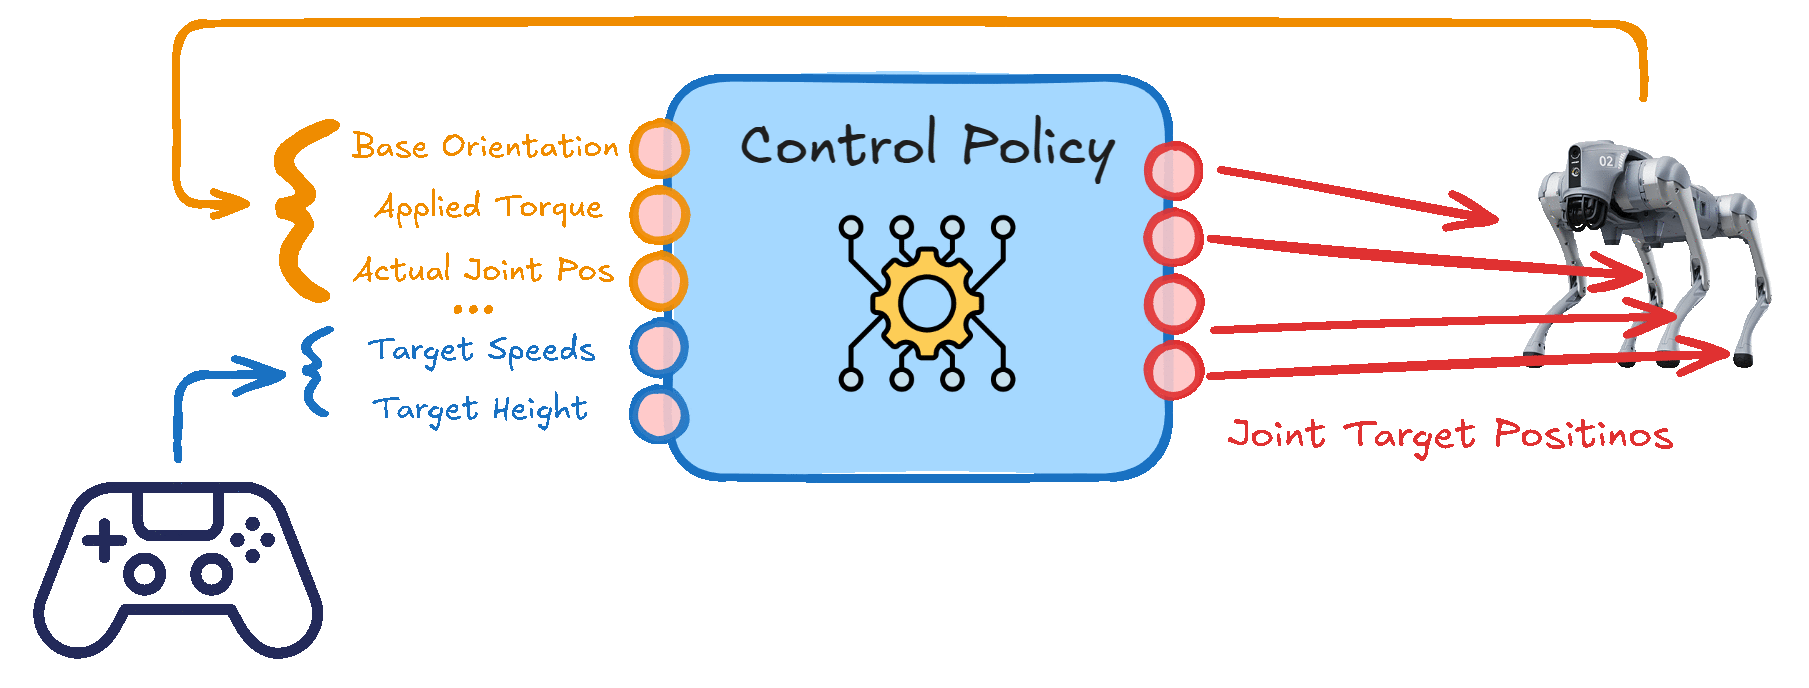
\includegraphics[width=0.9\linewidth]{fig/policyaa_2}
	\end{subfigure}
	\caption{Example of input-output mapping in a neural network for policy learning.}
\end{figure}

Once the environment is established, it is critical to consider how states, actions, and rewards are designed for effective learning. The state typically includes proprioceptive information, such as joint angles and velocities. Actions correspond to the motor commands needed to drive the robot’s joints, which the policy must produce in response to incoming observations. The reward function is designed to incentivize stable and efficient locomotion, often emphasizing forward progress, energy efficiency and reduced body tilt or impact forces. By balancing these elements, the policy gains a clear sense of what behaviors are desirable and how to achieve them through repeated interaction with the environment.

The reinforcement learning framework itself, such as Proximal Policy Optimization (PPO), serves as the computational spine of the training process. Through iterative updates, it refines the neural network underlying the control policy, assigning suitable weights to different components of the input data. In this network, hidden layers progressively extract relevant features, culminating in outputs that specify joint commands for each gait cycle. Over time, the network learns to anticipate how minute changes in posture or velocity will affect overall stability, enabling smoother and more adaptive movements.

In conclusion, creating a robust control policy for quadruped robots involves much more than a single algorithmic trick. It requires constructing a high-fidelity environment, defining state and action spaces that accurately capture the robot’s capabilities, and training with a clear reward function that drives the policy toward favorable outcomes.